% !TeX root = ../main.tex

\chapter{绪论}

\section{课题研究背景}

\subsection{加速器控制系统简介}
粒子加速器是利用电磁场不断加速真空环境下的带电粒子,使之达到很高能量的装置。粒子加速器广泛应用于基础科学、生产生活、医疗卫生等各个领域\cite{hong2014,Clayton2015}。同步辐射是速度接近光速的带电粒子在电磁场的作用下发生弯转时,沿弯转轨道的切线方向发出的电磁辐射,最早是在电子同步加速器上发现的。同步辐射光源是指产生同步辐射的物理装置,它的主要设备包括注入器和电子储存环,注入器产生电子束并将其加速到所需能量,电子储存环使得电子发生弯转并产生同步辐射光。同步辐射光具有亮度高、强波长范围宽且连续可调、方向性及偏振性好、超纯净等优异特性,广泛应用于物理、化学、材料科学、生命科学、环境科学、微电子等众多基础研究和应用研究领域。

粒子加速器是复杂系统的精密集成,通常粒子加速器会包括电子枪、磁铁、电源、真空、微波高频、束流注入引出、束流测量和冷却水等多个系统,系统之间协调工作,才能保证加速器的正常工作,这是加速器控制系统首先要实现的功能。加速器运行期间,需要密切监测各个系统的工作状态,进行必要的联锁和保护,才能够保证加速器安全、稳定和高效的运行。加速器运行状态监测和联锁保护,也是加速器控制系统必需的功能。综上所述,加速器控制系统承担着加速器“大脑”的功能,直接指挥着加速器的调试、运行。一般来说,粒子加速器控制系统的具体任务如下\cite{zhao2006,Liu2006}:

\begin{enumerate}[itemindent=1em,label=(\arabic*)]
	\item 对电子枪、磁铁电源、真空、高频、微波、束调管、注入、冷却水、插入件以及束测等系统的设备进行监测和控制;
	\item 建立报警和联锁保护机制,确保操作人员和设备的安全;
	\item 提供定时及同步系统,实现相关设备间协调工作及信号同步;
	\item 建立上层物理应用软件,实现轨道校正、BBA、线性参数测量与校正、响应矩阵测量、局部凸轨、Lattice标定、束流光学参数测量及校正、插入,元件补偿、装置状态和参数分析等功能;
	\item 建立数据存档和查询系统,以网页方式提供历史数据查询与分析等功能。
\end{enumerate}

粒子加速器往往体积庞大、设备众多,其控制系统一般是基于网络的分布式控制系统,目前国内外应用最为广泛的控制系统开发工具是EPICS。EPICS是实验物理和工业控制系统(Experimental Physics and Industrial Control System)的缩写,是20世纪90年代初发展起来的大型分布式控制系统的软件运行环境和开发平台,已成功应用于全世界上百个大科学装置,涉及大型粒子加速器、高能物理探测器、大型天文望远镜等多种类型装置\cite{EPICS}。国际上,European XFEL、NSLS-II、ITER、LCLS-II、FRIB、ESS、ILC等工程项目都采用EPICS作为控制系统的软件开发平台\cite{Aghababyan2015,Carcassi2009,Wallander,Flath2017,Shen2016,Arredondo2013,carwardine-2007}。在国内,EPICS已成功应用于近年来相继完成的HLS-II、北京正负电子对撞机重大改造项目(BEPC-II)、上海同步辐射光源(SSRF)、中国散列中子源(CSNS)等大型科学工程项目\cite{liweimin-control-2007, Zhao2007,Shen2010,C.H.Wang2011},目前正在建设中的上
海硬X射线自由电子激光装置(SHINE)和高能同步辐射光源(HEPS)等项目也采用EPICS作为控制系统的软件开发平台\cite{Lv2018a,Chu2018a}。EPICS控制系统是基于网络的分布式控制系统,其架构如图~\ref{fig:epics-control-system-arch}所示,遵循所谓的“标准模型”(Standard Models)\cite{Kuiper1991},从上到下分为三层,分别为管理层(Supervisory controls)、前端控制层(Front End Controls)和设备控制层(Devices Controls)。

\begin{figure}[!htb]
	\centering
	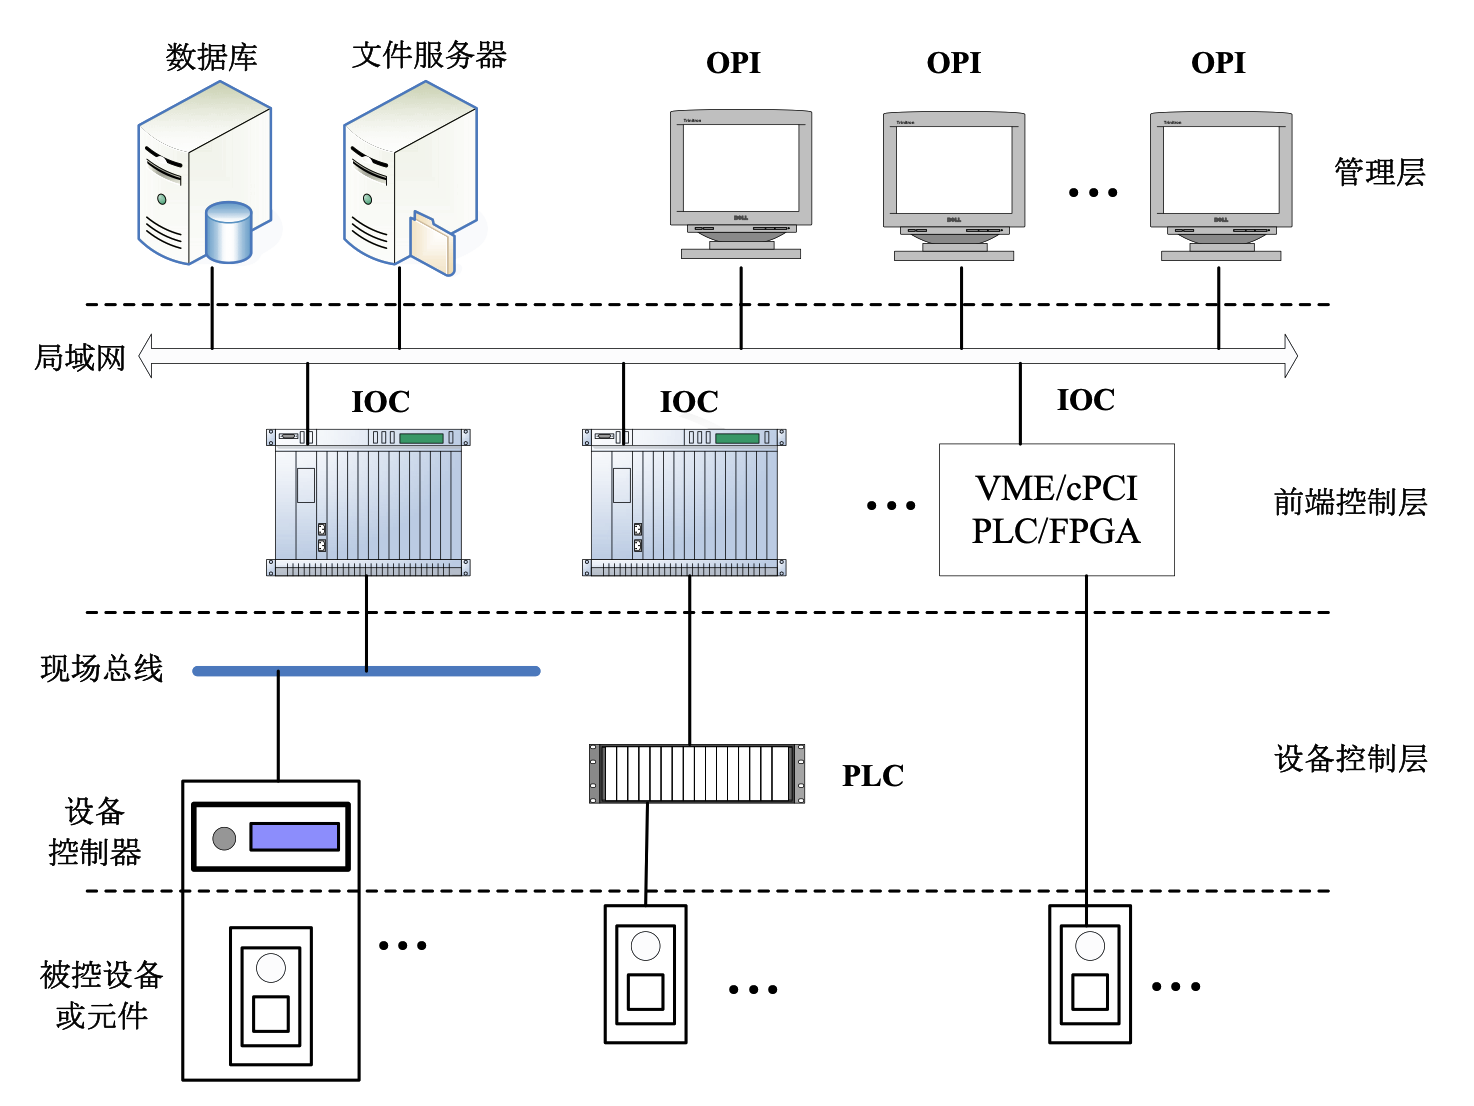
\includegraphics[width=\textwidth]{epics-control-system-arch.png}
	\caption{基于EPICS的控制系统基本结构图}
	\label{fig:epics-control-system-arch}
\end{figure}

\begin{itemize}
	\item \textbf{管理层(Supervisory controls)} \\ 
	位于系统最上层是管理层,由OPI和服务器系统组成。其中,OPI给操作人员提供了交互界面,操作人员通过OPI监控系统状态,发送控制命令。服务器系统包括数据库、文件服务器等,提供系统初始化配置、历史数据存档和查询等功能。
	\item \textbf{前端控制层(Front End Controls)} \\ 
	前端控制层在EPICS控制系统中处于关键位置,它与管理层构成客户端/服务器(Client/Server)模式,前端控制层为服务端,管理层为客户端,二者之间通过Channel Access(CA)通信协议进行通信。前端控制器(也被称为IOC)负责输入输出控制、保存动态数据和控制算法,是控制任务的主要执行者。同时,通过CA协议将相关信息发布至管理层。
	\item \textbf{设备控制层(Devices Controls)} \\ 
	位于系统最底层的是设备控制层。被控设备种类多样,有嵌入式智能设备控制器,负责控制功能复杂的设备,它们可以通过现场总线、以太网与IOC通信;也可以是PLC,用来对下层设备进行过程控制和状态监测,PLC可以通过网络或串口的方式与IOC通信。除此之外,IOC也可以通过IO模块直接对设备和元件进行控制。
\end{itemize}

合肥光源是国家同步辐射实验室建设的我国第一台以真空紫外和软X 射线为主的专用同步辐射光源,在1989年建成出光。合肥光源建成之后经历了2次改造,分别是国家同步辐射实验室二期工程(1998年\textasciitilde2004年)和合肥光源重大维修改造(2010年\textasciitilde2014年)。合肥先进光源(Hefei Advanced Light Faculty,HALF)是由国家同步辐射实验室提出的第四代基于衍射极限储存环的同步辐射光源。在中国科学院、安徽省、合肥市的支持下,HALF预研工程于2017年底启动,将对加速器、光束线站的核心关键技术进行攻关及样机研制。HALF工程计划于2020年完成。本论文的研究内容是HALF预研工程子项目“加速器控制技术”的一部分,研究成果可以作为HALF建设的技术储备。

\subsection{实时性分类和实时以太网}
实时性的含义是一个事件发生后,在确定时间内系统做出反应的能力。对于工业自动化系统来说,实时性是工业控制网络的基本要求,根据不同的应用场合,将实时性要求划分为三个范围,分别为:

\begin{enumerate}[itemindent=1em,label=(\arabic*)]
	\item 信息集成和较低要求的过程自动化应用场合,实时响应时间的要求是100ms或更长;
	\item 绝大多数的工厂自动化应用场合,实时响应时间的要求最少为5\textasciitilde10ms;
	\item 对于高性能的同步运动控制应用,特别是在100 个节点下的伺服运动控制应用场合,实时响应时间要求低于1ms,同步传送和抖动时间小于1$\mu$s\cite{liao-2005}。
\end{enumerate}

工业以太网是指用于工业自动化环境,符合IEEE 802.3标准,按照IEEE 802.1D和IEEE 802.1Q规范,但没有进行实时性扩展而实现的以太网。工业以太网的实时响应时间可以达到5\textasciitilde10ms,相当于现有的现场总线。对于一些实时性能要求更高的应用场合,各标准组织和公司基于工业以太网提出了各种提升实时性能的技术方案。这些方案都在IEEE 802.3标准的基础上对其进行了实时性扩展从而提高实时性能,这就是实时以太网(Real Time Ethernet,RTE)。

实时以太网是指在不改变ISO/IEC8802-3的通信特征、相关网络组件或 IEC1588 的总体行为基础上,通过一定程度的修改,使之满足实时行为。实时以太网既保持了普通以太网高通信速率等优势,又提高了其实时性、确定性、可靠性\cite{Hao2018}。根据实现机制和工业控制领域的实时性等级,实时以太网可以划分为class A、class B和class C三类\cite{wei2013},如图~\ref{fig:real-time Ethernet kinds}所示,一种实时以太网可以同时支持不同的技术实现方案,例如Ethernet/IP既有支持Class A的方案,也有支持Class C的方案。
Class A类别的实时以太网保持TCP/IP协议簇不变,保留传输层及以下的协议,只在应用层做了实时性修改,所以这种协议虽然可以直接接入普通以太网,但是并未克服普通以太网的原有缺陷,实时性不高,Modbus/TCP和Ethernet/IP实时以太网属于Class A类型的协议。Class B类别实时以太网弃用了TCP/IP的传输协议,在数据链路层及以上使用自定义的数据通信机制,物理层使用标准以太网的通信硬件,该类别实时以太网的实时性较强,一般可满足高性能的同步运动控制应用的实时需求,POWERLINK和PROFINET RT等实时以太网属于Class B类型的协议。Class C类别的实时以太网在数据链路层使用自定义的数据通信机制的同时,在物理层使用了专用的网络通信硬件,该类别实时性能最好,EtherCAT和PROFINET IRT等实时以太网属于这类协议,Ethernet/IP为了提升性能,也有支持Class C类的技术方案。综合来看,在实时性能上,Class C优于CLass B,Class B优于Class A;在协议通用性上,Class A优于Class B,Class B优于CLass C。目前,在工业自动化领域有PROFINET、POWERLINK、SERCOS III、EtherCAT 及EtherNet/IP 5个主流的实时以太网技术,以下分别做简单介绍。

\begin{figure}[!htb]
  \centering
  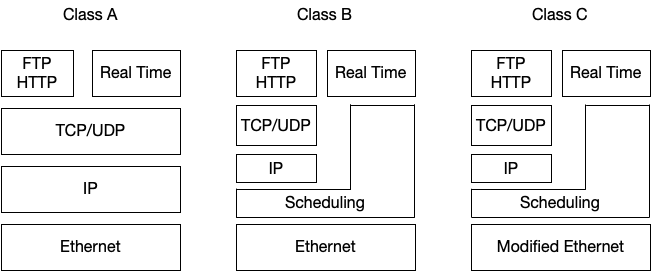
\includegraphics[width=\textwidth]{real-time-Ethernet-kinds.png}
  \caption{实时以太网分级}
  \label{fig:real-time Ethernet kinds}
\end{figure}

\subsubsection{POWERLINK}
POWERLINK最初由奥地利B$\&$R公司于2001年11月创立和开发,自2003年以来,由独立的用户组织Ethernet POWERLINK Standardization Group(EPSG)负责该技术的进一步发展\cite{ESPG}。EPSG在2008年发布了POWERLINK技术的开源版本openPOWERLINK,可在 PC、PLC、FPGA等硬件平台上实现\cite{oplk}。POWERLINK遵循IEEE1588分布式时钟系统标准,在数据链路层采用SCNM(Slot Communication Network Management)时间分片网络管理机制避免数据冲突从而进行高效的数据传输。

\subsubsection{PROFINET}
PROFINET是由 Profibus International 组织提出的实时以太网通信协议,基于IEEE 802.1D和IEEE 1588标准进行实时扩展\cite{Feld2005}。为满足不同工业场景下实时性需求,PROFINET提供了一个标准通信协议和RT、IRT两种实时通信协议。标准通信协议是基于TCP/IP的协议,主要用于设备的参数化配置、组态和诊断数据的读取。RT是软实时协议,根据IEEE 802.1p标准定义了报文的优先级,主要用于数据的高性能循环传输。IRT协议的实现需要专用的等时同步ASIC芯片,适用于高性能数据传输和同步运动控制应用等场合。

\subsubsection{EtherCAT}
EtherCAT由德国Beckoff公司研发,由EtherCAT Technology Group(ETG)组织维护发展。EtherCAT采用IEEE 1588标准实现分布式时钟精确同步,用于现场级的高速I/O网络\cite{Wang2011}。EtherCAT采用集总束帧等时通信的模式,主站负责把数据帧发送给各个从站,每个从站从该帧中取走属于自己的数据,或者写入该从站要输出的数据。从站在处理完成后会修改标志位,表明已完成数据帧的处理。

\subsubsection{SERCOS III}
SERCOS III是串行实时通信系统(Serial Real-time Communication System,SERCOS)的第三代协议,主要用于实现工控机与数字伺服系统、传感器和可编程控制器I/O口之间的实时数据通讯\cite{Wang2017}。SERCOS III采用集总束帧等时通信模式,与EtherCAT的通信模式相同。SERCOS III协议的通信循环周期最快可达到31.25$\mu$s,但必须使用专用的SERCOS接口控制芯片。

\subsubsection{EtherNet/IP}
Ethernet/IP(Ethernet/Industrial Protocol)是由ControlNet International(CI)、Industrial Ethernet Association(IEA)和Open DeviceNet Vendor Association(ODVA)共同研发的,在标准的以太网硬件上运行,在应用层采用CIP(Common Industrial Protocol)协议来进行实时数据交换\cite{Paul2001}。Ethernet/IP为了提升性能,也有支持Class C类的技术方案,通过专用芯片可以将EtherNet/IP的循环周期缩短到到百微秒量级。

\begin{table}[!hbt]
  \centering\small
  \caption{5种主流工业以太网性能比较}
  \label{table:1.1} 
  \begin{tabular}{cccccc}
    \toprule

     &POWERLINK&PROFINET& EtherCAT &SERCOS III&EtherNet/IP\\
    \midrule
    发布时间& 2001& 2006 &2003& 2008& 2006\\
    
    冗余支持  &是& 是 &  否  &是  &是\\
    
    应用层协议 & CANopen&  Profibus&    CANopen&  SERCOS  &DeviceNet\\
    
    交叉通信  &是  &是  &   否 &否  &是\\
    
    循环周期  &100μs& 100μs&  100μs &100μs& 100μs\\
    
    抖动  &50-80ns & 20ns& 20ns  &50-80ns  &100ns\\
    
    技术实现& 无ASIC& ASIC&  ASIC  &ASIC&  无ASIC\\
    
    开放性 &主从开放 &从站开放&需购买授权 &主从开放 &主从开放\\
    
    通信模式  &轮询机制 &轮询机制&  集束帧&  集束帧 &轮询机制\\
    
    时钟标准& IEEE1588& IEEE1588& IEEE1588& IEEE1588& IEEE1588\\
    
    安全支持& openSAFETY &ProfiSafe &FEoE &SERCOS Safe& CIP Safety\\                  
    \bottomrule
  \end{tabular}

\end{table}

表~\ref{table:1.1}列出了5种主流工业以太网协议的性能。从表中可以看出,5种主流实时以太网技术在实时性方面的性能相当,循环周期都达到了100$\mu$s量级,可以满足加速器装置控制系统中对实时性的大部分需求。值得指出的是,在这5种主流实时以太网技术中,只有POWERLINK是完全开源的技术。


\subsection{加速器控制系统中的实时性需求}

对于加速器控制系统来说,大部分系统对实时性的要求并不高,相当于工业自动化系统的第一类场合,实时响应时间的要求是100ms或更长,如恒温水系统的监控、真空状态的监测、人身安全保护系统等;慢联锁保护系统的实时响应时间在10ms量级,相当于工业自动化系统的第二类场合;对实时性要求较高的系统则与工业自动化系统第三类场合的要求类似或更高,如快联锁保护系统和电子储存环轨道快反馈系统(Fast Orbit Feedback,FOFB)等。

慢联锁保护系统的实现方式大都采用PLC作为控制器,PLC间的通信采用一般采用实时以太网,如ALBA和SSRF的慢联锁保护系统\cite{Alba-eps,yu2020},但LCLS的联锁系统的响应时间小于工作周期8.333ms,采用的是自己研发的FPGA控制器,节点间通过自主设计的实时通信协议进行通信\cite{Norum-2009}。

快联锁保护系统的实时性要求在10$\mu$s量级,一般用于束流丢失的机器保护,其实现方式因应用场合的不同而有所差异。例如上海光源的束流丢失保护系统采用集中控制方式,将所有140个BPM信号汇总到NI PXI的FPGA板卡中,以提高系统的实时性\cite{SSRF};西班牙ALBA的束流丢失保护系统采用了专门设计的技术,将MRF定时技术的单向数据传输改进为双向数据传输,以实现高的实时性\cite{Alba-eps}。


电子储存环轨道快反馈频率达kHz量级,反馈周期为ms量级,不同的装置所采用的方法差异较大。例如,上海光源轨道快反馈系统曾经采用反射内存方式在10个站点间共享数据,每个站点采用2台VME计算机,分别用作轨道数据的采集和反馈校正\cite{SSRF};英国Diamond轨道快反馈系统采用RocketIO来构建数据传输网络,通信速度是2.12Gbps\cite{DIAMOND-FOFB};美国NSLS-II轨道快反馈系统采用自主研发的串行通信接口SDI在30个计算节点间传输数据,系统快反馈频率可以达到10kHz\cite{NSLS-II-FOFB}。

从上述的解决加速器装置控制中高实时性问题的技术路线来看,有的采用自主设计的专用通信方案\cite{Norum-2009},有的采用实时以太网等通用技术\cite{Alba-eps}。一般来说,通用技术较专用技术具有更好的开放性和灵活性,并可以节省产品的开发成本,缩短开发周期。因此,应该在粒子加速器控制领域中加强对实时以太网技术的研究和应用。

POWERLINK作为一种开源的实时以太网技术,其开源性对加速器装置控制系统来说具有特别重要的意义。开放和共享一直是加速器控制系技术的发展方向,现在流行的控制系统开发平台无一例外都是开源的,如EPICS、TANGO、DOOCS等\cite{TANGO,DOOCS}。

\section{国内外研究现状}
POWERLINLK已在工业控制领域得到了广泛的研究和应用\cite{xu-2015,zhu-2014,shi-2012,huang-2012,Seno-2007,cena-2009},目前在加速器控制领域,与POWERLINK相关的研究和应用还很少。国际上只有西班牙ALBA将POWERLINK用于设备保护系统,国内只有上海光源在开发光束线前端真空泄露快保护系统时,控制器间的通信设计参考了POWERLINK的通信方式。而在应用最广泛的EPICS系统中,目前还未见与POWERLINK相关的文献。

\subsection{基于POWERLINK的ALBA设备保护系统}
ALBA是一台三代同步辐射光源,建造于西班牙的巴塞罗那,于2012年建成投入使用。ALBA由直线加速器、满能量增强器和储存环组成,其中电子储存环的能量为3GeV,周长为270米,直线加速器产生并加速电子束流至100MeV,低发射度的增强器加速电子束流至满能量3Gev。ALBA目前拥有八条光束线,包括软X射线和硬X射线,主要用于生物科学、凝聚态物质、纳米科学和材料科学的研究。ALBA的设备保护系统的任务是避免装置设备受到损害。

ALBA的设备保护系统采用B$\&$R公司的X20CP1484型号PLC作为控制器,采用分布式I/O模块作为现场设备,其硬件架构如图~\ref{fig:alba-eps-arch}所示。负责加速器设备保护的PLC共有56台,PLC之间的通信周期要求达到20ms以下,采用百兆以太网POWERLINK技术实现。分布式I/O模块安装在加速器隧道内的铅屏蔽箱中,共有110个I/O模块通过X2X总线与PLC通信\cite{Alba-eps}。PLC通过以太网接入基于Tango的ALBA主控制系统局域网中,一台Tango的设备服务器通过基于TCP/IP的Mobus协议来轮询PLC,从而监控设备保护系统的状态。

\begin{figure}[!htb]
	\centering
	
\includegraphics[width=\textwidth]{alba-eps-arch.png}
	\caption{ALBA设备联锁保护系统架构图}
	\label{fig:alba-eps-arch}
\end{figure}

ALBA的设备保护系统主要包括六个子系统,分别是:真空、磁铁、射频、插入件、前端设备和光束线。每条光束线都有一个独立的设备保护系统系统,并全部接入到加速器的设备保护系统中。每个子系统除了本地保护逻辑之外,当子系统中某些设备状态异常时时,设备保护系统应立即通知其他相关子系统做出保护动作。例如,当真空阀由于真空管道中的压力超过阈值而关闭时,设备保护系统应立即关闭高频系统并切断束流。每个子系统由相关PLC负责,子系统之间的联锁信号都是通过POWERLINK进行传输。


\subsection{CERN在辐射区域关于POWERLINK的应用研究}
欧洲核子中心(Conseil Européenn pour la Recherche Nucléaire,CERN)位于瑞士日内瓦,是世界上最大的粒子物理实验室,建设了包括周长26.7千米的大型强子对撞机(Large Hadron Collider,LHC)、周长6.9千米的超级质子同步加速器(Super Proton Synchrotron,SPS)等多个加速器和一个反质子减速器 (Antiproton Decelerator,AD)。

CERN加速器装置控制系统的硬件架构可以分成三层,分别是前端层、现场总线层和分布式I/O层,如图~\ref{fig:cern-hardware-arch}所示。其中,前端层是PLC、VME、PICMG 1.3、MTCA.4等总线控制器,控制器通过现场总线和工业以太网来对分布式I/O层的不同设备进行控制。CERN现场总线层的通讯需求如表\ref{table:1.2}所示,CERN在不同区域内采用了不同的通信技术,在无辐射区域采用Profibus总线和Profinet工业以太网技术,对靠近LHC装置的辐射区域则采用耐辐射的WorldFIP总线技术\cite{Daniluk2017}。

\begin{figure}[!htb]
	\centering
	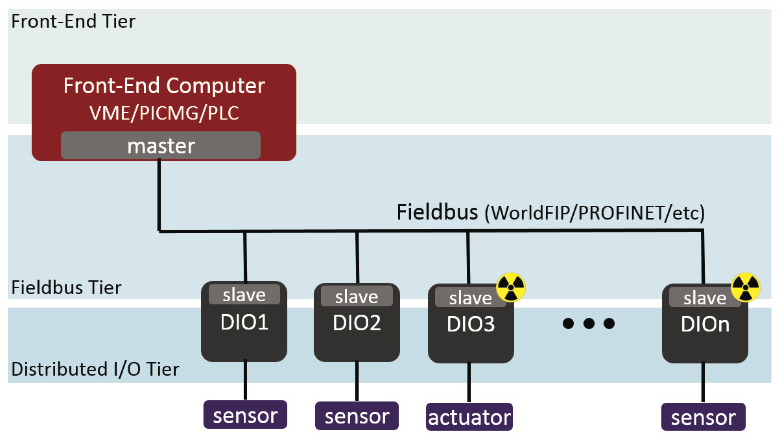
\includegraphics[width=0.75\textwidth]{cern-hardware-arch.png}
	\caption{CERN的硬件架构图\cite{Daniluk2017}}
	\label{fig:cern-hardware-arch}
\end{figure}

\begin{table}[hbt]
  \centering
  \caption{CERN现场总线层的通讯需求\cite{Daniluk2017}}
  \label{table:1.2}
  \setlength{\tabcolsep}{15mm}
  \begin{tabular}{cc}
    \toprule

    characteristic & value\\
    \midrule
    topology & mainly daisy chain\\
    
    nodes & 100\\
    
    cycle time & 1ms\\
    
    synchronization  & 100μs\\
    
    data-per-cycle & 1Kbyte\\              
    \bottomrule
  \end{tabular}

\end{table}

在CERN的最新研究计划中,在现场总线层加入了POWERLINK实时以太网技术。POWERLINK作为唯一开源的可支持多种平台实时以太网技术,完全满足表\ref{table:1.2}所示的通讯需求。目前,CERN已在现有芯片如NetX52上实现了Profinet、POWERLINK等四种实时以太网协议,但是现有芯片不能工作在辐射区域内。CERN计划在辐射区域内采用Microsemi公司的耐辐射FPGA芯片来实现POWERLINK协议,直接可以与无辐射区域的支持POWERLINK的现有芯片直接通信。这种升级不需要替换所有已安装的设备,极大节省了人力物力。

\subsection{上海光源的光束线前端真空泄漏快保护系统}
上海光源是我国建造的第一台第三代中能同步辐射光源,由一台150MeV的直线加速器,输运线,将电子束加速到到3.5GeV的满能量增强器,周长432米的3.5GeV电子储存环、光束线和实验站组成。光束线由安装在真空室中的一系列光学元件组成,在加速器正常运行期间,光束线的真空室是对储存环开放的。当光束线发生真空泄漏事故时,为防止真空泄漏扩散,真空保护快阀必须立即关闭。由于同步辐射光的直接照射会打坏真空保护快阀,因此必须在真空快阀关闭前,切断储存环的束流。位于光束线接口处的真空泄漏快保护系统作为整个光源机器保护系统的一部分,需要在真空泄漏信号给出后1ms内切断储存环束流。

上海光源的光束线前端真空泄漏快保护系统的IO站点数为20,需要是在1ms内,完成所有IO站点的之间的实时数据传输\cite{liu-2010}。系统内各节点的硬件平台是FPGA和实时以太网,通讯协议的设计参考了实时以太网POWERLINK的PRC(PollResponse Chaining)通讯模式,按照时间分片的原理来传输实时数据,各从站在被分配的时间片内传输数据,从而避免通信冲突,通信机制如图~\ref{fig:time-slice-principle}所示。

\begin{figure}[!htb]
	\centering
	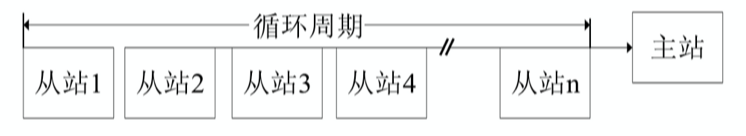
\includegraphics[width=0.6\textwidth]{time-slice-principle.png}
	\caption{时间分片原理图}
	\label{fig:time-slice-principle}
\end{figure}

第一阶段,主站的时钟与所有从站时钟同步。第二阶段,在传输数据的第一个循环周期内,先进行主时钟与第一个节点时钟的同步,再按照时间分片原理进行数据传输;在第二个循环周期内,先进行主时钟与第二个节点时钟的同步,再按照时间分片原理进行数据传输;在n+1个循环周期内,先进行主时钟与第一个节点时钟的同步,再按照时间分片原理进行数据传输,依次类推。


\section{论文工作的主要内容及创新点}

本论文的主要研究内容为实时以太网POWERLINK在粒子加速器控制系统中的应用研究。首先,我们将对加速器控制系统中实时性需求进行详细分析,并调研POWERLINK在国内外加速器控制系统中的应用,然后开展对POWERLINK通信协议的研究,解析POWERLINK协议并进行POWERLINK性能测试,根据实测参数发展了理论分析和仿真建模两种方法对POWERLINK通信周期进行估算;其次在EPICS环境下基于POWERLINK设计分布式IO系统,开发基于Zynq的控制器以及EPICS设备驱动程序;然后我们搭建相应的测试系统并进行相关实时性能测试,根据实测参数进一步完善了理论计算和仿真建模方法;最后,基于POWERLINK和zynq控制器设计了HALF设备保护系统,并通过理论分析和仿真建模两种方法来估算技术方案的可行性。

本文分为五个章节,每章节的主要内容的简介如下:

第一章为绪论。本章介绍了课题研究背景,包括加速器控制系统简介、实时性分类、实时以太网以及加速器控制系统的实时性需求。然后进行了国内外研究现状调研,包括基于POWERLINK的ALBA设备保护系统、CERN在辐射区域关于POWERLINK的应用研究和上海光源的光束线前端真空泄漏快保护系统。最后描述了本课题的创新点。

第二章为POWERLINK通信协议研究。本章首先介绍了POWERLINK实时以太网技术,包括POWERLINK协议的通信机制、网络模型和数据帧结构。然后介绍了POWERLINK的实现方式,包括基于Linux实现POWERLINK协议和基于FPGA实现POWERLINK协议。最后根据系统实测参数,发展了理论分析和仿真建模两种方法对POWERLINK通信周期进行估算。

第三章为EPICS环境下基于POWERLINK的分布式IO系统的设计与性能分析。本章首先介绍了基于千兆POWERLINK的系统设的分布式IO系统的设计与开发,搭建了测试系统,进行了性能测试。然后对系统测试结果进行了分析,提出了改进方案,搭建了新的系统并进行了性能测试。最后基于改进方案的系统测试结果,我们进一步完善了理论计算和仿真建模两种方法。

第四章为HALFF设备联锁系统的设计。本章首先介绍了HALF目前的设计方案,并对国内外加速器装置设备保护系统进行了调研,基于千兆POWERLINK和Zynq控制器设计了HALF设备保护系统,然后通过理论计算和仿真建模估算了HALF设备保护系统设计方案的实时性能。最后我们对HALF设备保护系统的信息报警和历史数据存档与查询系统进行了设计。

第五章为论文的工作总结与展望。


本文的主要创新点为:
\begin{enumerate}
	\item 基于Zynq控制器实现了千兆POWERLINK通信协议,并通过自主开发的驱动程序,首次将POWERLINK集成EPICS架构中,提高了数据通信的实时性能,拓展了EPICS的应用范围。
	\item 基于千兆POWERLINK技术和Zynq控制器设计了HALF设备保护系统,并通过理论计算和仿真建模两种方法估算了设计方案的实时性能。
\end{enumerate}

